\documentclass[aspectratio=169]{beamer}
\usepackage[utf8]{inputenc}

\setbeamersize{text margin left=3mm,text margin right=3mm} 

\usetheme{Oxygen}
\usepackage{graphicx}
\usepackage{hyperref}
%\usepackage{movie15}
\usepackage{textpos}
\usepackage{fancybox}
\usepackage{colortbl}
\usepackage{rotating}
\usepackage{subfigure}
%\usepackage{subcaption}
\usepackage{multicol}
\usepackage{multirow}
\usepackage{amsmath,amssymb,amsfonts,amsbsy,dsfont}
\usepackage{mathrsfs}
\usepackage{amsthm}
\usepackage{bm}
\usepackage{array}
%\usepackage[caption=false]{subfig}
\usepackage{arydshln}
\usepackage{breakcites}
\usepackage{booktabs}

\let\oldcite\cite % store the original \cite command
\renewcommand{\cite}[1]{{\tiny\oldcite{#1}}}

\usepackage{bm}
\providecommand{\mat}[1]{{\bm{#1}}} 
\providecommand{\ve}[1]{{\bm{#1}}} 


\newcommand{\x}{\negthinspace\times\negthinspace}
\usepackage{etoolbox}

\DeclareUnicodeCharacter{2212}{-}


\usepackage[nopar]{lipsum} 

\newif\ifcomment
\newcommand{\Com}{\par\footnotesize\itshape\commenttrue}

\newenvironment{Itemize}
 {%
  \edef\Itemizecurrent{\the\font}%
  \itemize
  \preto{\item}{\ifcomment\par\Itemizecurrent\fi}%
 }{%
  \enditemize
 }


%%%%%%%%%%%%%%%%%%%%%%%%%%%%%%%%%%%%%%%%%%%%%%%%%%%%%%
%%%%%%%


\title[A Deep Learning Approach for Image-based Semantic Segmentation with Preserved Interpretability | Juan Carlos Aguirre Arango]{A Deep Learning Approach for Image-based Semantic Segmentation with Preserved Interpretability}


\author{\normalsize{Juan Carlos Aguirre Arango}\\ \scriptsize{jucaguirrear@unal.edu.co
}}

\institute{\includegraphics[width=0.15\textwidth]{EscudoUN.png}\\\scriptsize{
Universidad Nacional de Colombia \\ Signal Processing and Recognition Group - SPRG
\\
Advisor: Andrés Marino Álvarez Meza, Ph.D.\\
Co-advisor: César Germán Castellanos Domíguez, Ph.D.\\
\vspace{-0.3cm}
}}
\date[]{\scriptsize{\today}}
%%-------------------------------------------------------------------
%% Options
%%-------------------------------------------------------------------
\setbeamercovered{dynamic}
\setbeamertemplate{navigation symbols}{}



\begin{document}

{\setbeamertemplate{headline}{}
\setbeamertemplate{footline}{}
\begin{frame}{}
\vspace{-0.7cm}
    \titlepage 
\end{frame}
}


\frame
{ \frametitle{Outline}
{\small 
  \tableofcontents[]}
}

\AtBeginSection[]
{
  \begin{frame}
  \frametitle{Outline}
  \tableofcontents[currentsection]
  \end{frame}
}



%%%%%%%%%%%%%%%%%%%%%%%%%%%%%%%%%%%%%%%%%
\section[Motivation]{Motivation}


\begin{frame}{Classic Machine Learning vs. Deep Learning}

\begin{figure}
    \centering
 \includegraphics[width=1\linewidth]{Figures/deep_examples.pdf}
    %\caption{Caption}
    \label{fig:enter-label}
\end{figure}




\end{frame}






\begin{frame}{Semantic Segmentation (SS)}
    

\begin{figure}
    \centering
    \includegraphics[width=0.58\linewidth]{Figures/segmentaitonDef.pdf}
    %\caption{Caption}
    \label{fig:enter-label}
\end{figure}

\begin{centering}
    \textcolor{blue}{Deep learning models have allowed the use of semantic segmentation \\ in multiple tasks} \cite{electronics11121884}

\end{centering}

\begin{columns}


\column{0.5\textwidth}


\begin{itemize}

    \item Autonomous Vehicles \cite{cakir2022semantic, s23020895, technologies10040090, Burel2022ImprovingDF}
    \item Virtual Reality \cite{9319081, 10.1145/2992138.2992144}
    

\end{itemize}

\column{0.5\textwidth}

\begin{itemize}
    \item Health care  \cite{QURESHI2023316, WOS:000673109800001,9804867}
    \item Agriculture \cite{LUO2023, 9395478}
    \item Satellite Imagery \cite{lilay2023semantic, WIELAND2023113452}
\end{itemize}



\end{columns}

\end{frame}

\begin{frame}{ Main Tasks in Medical Image Analysis \cite{li2021systematic}}


\begin{columns}
\column{0.5\textwidth}


 \begin{figure}%[H]
    \begin{centering} \includegraphics[width=1\textwidth]{Figures/seg_graph.png}
    \end{centering}
\end{figure}

  \column{0.5\textwidth}
Most diagnosis methods rely on changes in morphological information of the region of interest \cite{kriti2022characterization}.

\vspace{0.5cm}

\textcolor{blue}{Small sample sizes and heterogeneous regions of interest are presented in medical image} \cite{CASTIGLIONI20219}. 


 \end{columns}
\end{frame}

% \begin{frame}{Interpretability}

% \begin{itemize}
%     \item  System understanding \cite{teng2022survey, xu2023interpretability, kolyshkina2021interpretability, bennetot2022practical}.
%     \item Use of medical image systems with confidence \cite{MARKUS2021103655, amann2020explainability}
%     \item Identify potential biases \cite{gilpin2018explaining, linardatos2020explainable}
% \end{itemize}



% \begin{figure}
%     \centering
%     \includegraphics[width=0.8\linewidth]{Figures/intermov.pdf}
% \end{figure}

% \textcolor{blue}{Complex and black-box nature of semantic segmentation models based on deep learning make their explainability challenging} \cite{linardatos2020explainable}. 

% \end{frame}


\begin{frame}{Signal Processing and Recognition Group - SPRG}
\begin{itemize}
    \item The SPRG is interested in developing machine learning systems to analyze biosignals \cite{BRON2015562, jimenez20183d,jimenez2021}. 
    \item Nowadays, the SPRG is developing \textcolor{blue}{objective and low-cost monitoring procedures for obstetric patients under regional neuraxial analgesia}.
\end{itemize}


\begin{figure}
    \centering
    \includegraphics[width=0.7\linewidth]{Figures/ses_unal_utp.pdf}
    %\caption{Feet thermal image example.}
\end{figure}

\end{frame}

\begin{frame}[allowframebreaks]{Childbirth Pain Monitoring}

Thermal imaging is an objective and non-invasive technique to quantify warm modifications after catheter placement due to blood flow redistribution~{\tiny{\cite{2143r23}}}. 

\begin{columns}
\column{0.5\textwidth}

\begin{figure}
    \centering
    \includegraphics[width=0.8\linewidth]{Figures/t20rainbow.jpg}
    \caption{Thermal imaging example.}
\end{figure}


\column{0.5\textwidth}

\textcolor{blue}{\textbf{Reliable and automatic thermal measurements are required during childbirth analgesia monitoring}} {\tiny{\cite{PMID:25232864}}}.


\end{columns}

\framebreak

\begin{figure}
    \centering
    \includegraphics[width=0.7\linewidth]{Figures/camaraLocation.pdf}
\end{figure}

\begin{center}
    \textcolor{blue}{Medical specialists from SES Hospital de Caldas designed a protocol of acquisition}
\end{center}
\end{frame}




\section{Problem Statement}


\begin{frame}{Issue \#1: Small Sample Size and Overfitting}

\begin{itemize}
\setlength\itemsep{1em}
    \item Challenges in acquiring sufficient datasets in obstetrics environments \cite{WOS:000754419000014, willemink2020preparing}
    \item Effective training requires extensive annotations \cite{sarker2021deep, li2021systematic}.
\end{itemize}

\begin{figure}
    \centering
    \includegraphics[width=0.4\textwidth]{overparametrized.png}
\end{figure}

\end{frame}


\begin{frame}{Issue \#2: High Variability in the ROI}

\begin{itemize}
\setlength\itemsep{1em}
    \item Variations in anatomy, pathology, and imaging parameters result in significant variations in the ROI's shape, size, and texture \cite{li2021systematic}.
    \item Diverse ROI positions can lead to images with different orientations, sizes, and shapes, even within the same subject. This variability includes cases where the ROI may overlap or be partially obscured \cite{arteaga2021segmentation}.
\end{itemize}
     
\begin{figure}
    \centering
    \includegraphics[width=0.5\textwidth]{Figures/high_roi_var.png}

\end{figure}

\end{frame}


\begin{frame}{{\fontsize{13pt}{13pt}\selectfont  Issue \#3: Lack of Quantitative Measures for Interpretability in SS Models}}

\begin{itemize}
\setlength\itemsep{1em}
    \item  Deep learning-based semantic segmentation models are often black-boxes, making their explanations challenging \cite{linardatos2020explainable}. 
    \item Current methods for explainability rely mainly on visual inspection or qualitative analysis, limiting the evaluation of model performance \cite{Wang_2022, salahuddin2022transparency}. 

    \begin{figure}
        \centering
        \includegraphics[width=0.61\textwidth]{Figures/lack_interpretability.pdf}
        
    \end{figure}
\end{itemize}

\end{frame}


\begin{frame}{Research Question}
    How can we develop a method for generating \textbf{local and equivariant representations} that can improve the \textbf{generalization} of \textbf{deep-learning} models while maintaining \textbf{interpretability} in \textbf{Semantic Segmentation} tasks for medical images?
\end{frame}



\section{Literature Review}

\begin{frame}{Small Sample size and
Overfitting}

\begin{figure}
    \centering
    \includegraphics[width=0.8\linewidth]{Figures/State-of-the-arr-obj1.pdf}
    %\caption{Caption}
    %\label{fig:my_label}
\end{figure}   

\begin{center}
    \textcolor{blue}{Random Fourier features bring properties of kernel methods within deep learning frameworks}    
\end{center}


\end{frame}

\begin{frame}{Kernel Methods}

\begin{figure}
    \centering \includegraphics[width=0.4\linewidth]{Figures/classic_kernels_view.pdf}
    \includegraphics[width=0.5\linewidth]{Figures/spacesHilbert.pdf}
\end{figure}


\begin{itemize}

    % accessible computacionalmente
    \item Kernel trick: $k(\mathbf{x},\mathbf{x}') = \langle \phi(\mathbf{x}), \phi(\mathbf{x}') \rangle_{\mathcal{H}} \ \ \
    \text{where}\  \phi: \mathcal{X} \rightarrow \mathcal{H}$

    \item Mercer condition: $\sum_{i=1}^n \sum_{j=1}^n k(\mathbf{x}_i,\mathbf{x}'_j) c_i c_j \geq 0$
    %EL problema se puede resolver


    % Nos permite construir duncional como una conbinacion lineal en el espacio proyectado
    \item Reproducibility: $f(\mathbf{x}) = \sum_{n=1}^{N} \alpha_n k(\mathbf{x}, \mathbf{x}_n) = \langle \boldsymbol{\omega}, \phi(\mathbf{x}) \rangle_{\mathcal{H}}$
\end{itemize}

\begin{center}
    \textcolor{blue}{It is difficult to scale kernel methods to large datasets}
\end{center}

\end{frame}


\begin{frame}{Bochner's Theorem and Random Fourier Features (RFF)}

A continuous function of the form $k(\mathbf{x},\mathbf{x}') = k(\mathbf{x}-\mathbf{x}')$ is a positive definite if only if $k(\mathbf{\delta})$ is the Fourier transform of a non-negative measure.

\begin{equation*}
    k(\mathbf{x}-\mathbf{x}') = \int_{\mathbb{R}^p} p(\boldsymbol{\omega}) \exp(j\boldsymbol{\omega}^\top(\mathbf{x} -\mathbf{x}')) d\boldsymbol{\omega} = \mathbb{E}_{\boldsymbol{\omega}}\big\{\exp(i \boldsymbol{\omega}^{\top}\mathbf{x}) \exp(-i \boldsymbol{\omega}^{\top}\mathbf{x})\big\}
    \label{equ:bochner}
\end{equation*}



 Where $\boldsymbol{\omega} \sim p(\boldsymbol{\omega})$

\vspace{0.9cm}


\begin{center}
    \textcolor{blue}{Allow us to find a representation where we can sample and get an approximation, named the RFF, for the mapping function in low dimensional space}
\end{center}

\begin{center}
    \textcolor{blue}{However, the RFF is limited for 1-D data, and if it is extended to 2-D, its parameters are not optimized through gradient descent}
\end{center}



\end{frame}


\begin{frame}{Characterization of
highly variable object patterns in CNN}
\begin{figure}
    \centering
    \includegraphics[width=0.75\linewidth]{Figures/State-of-the-ar-obj2.pdf}
    %\caption{Caption}
    %\label{fig:my_label}allows
\end{figure}    
\vspace{-0.7cm}
\begin{center}
    \textcolor{blue}{Encoder-decoder architectures allow capturing both context and location information}
\end{center}

\end{frame}

\begin{frame}[allowframebreaks]{Encoder-Decoder: Image-based Segmentation}


\begin{figure}%[H]
\begin{centering}
\includegraphics[width=0.35\textwidth]{Figures/tranlationEquivariance.pdf}
\par\end{centering}
\end{figure}

\begin{center}
    \textcolor{blue}{Translation equivariance and local properties of Convolutional layers make them efficient}
\end{center}

\framebreak

\begin{figure}
    \centering \includegraphics[width=1\linewidth]{Figures/encoder-decoder.pdf}
\end{figure}



\begin{center}
    \textcolor{blue}{Mismatch characteristics between encoder and decoder \cite{zhou2020unet, Wang2021}}
\end{center}

\end{frame}


\begin{frame}{ Quantitative Interpretability of SS models}
\begin{figure}
    \centering
    \includegraphics[width=0.75\linewidth]{Figures/State-of-the-ar-obj3.pdf}
    %\caption{Caption}
    %\label{fig:my_label}
\end{figure}    
\vspace{-0.7cm}
\begin{center}
    \textcolor{blue}{Still, quantitative measures for assessment interpretability are necessary}
\end{center}

\end{frame}


\begin{frame}{Class Activation Maps}

\begin{figure}
    \centering
    \includegraphics[trim={1.1cm 0 0 0},clip,width=0.72\textwidth]{Figures/camsSchema.pdf}

\end{figure}

\begin{center}
    \textcolor{blue}{CAMs provide visual inspection result analysis, with a primary focus on classification models that do not incorporate location-mask information}
\end{center}

\hfill \footnotesize{$\mathbf{A}$ and $\boldsymbol{\beta}$ are the feature maps, and the CAMS weights, respectively, $\odot$ stands for Hadamard product.}


\end{frame}


\section{Aims}

\begin{frame}{General Aim}
    Develop a deep-learning-based semantic image-segmentation methodology incorporating a \textbf{convolutional} layer based on \textbf{Random Fourier Features} and comprehensive \textbf{interpretability measures} to encode high variable and relevant patterns related to the region of interest and improve generalization performance under conditions of \textbf{scarce data}.
\end{frame}


\begin{frame}{Specific Aims}
   \begin{itemize}
    \setlength\itemsep{1em}

        \item To design an extension of \textbf{Random Fourier Features} for \textbf{spatial data} with optimization through \textbf{gradient descent} for generalization under \textbf{scarcity data} through \textbf{local and equivariant characterization}.

        \item To develop a \textbf{semantic segmentation} approach based on \textbf{encoder-decoder architectures} that incorporate Random Fourier Features for \textbf{enhanced skip representation} for improved capture of \textbf{small and variable} objects in semantic segmentation tasks.

 
        \item To develop a post-hoc \textbf{interpretability} approach based on measures for \textbf{quantitative assessment} of relevance maps taking into \textbf{account the spatial information} of semantic segmentation tasks for \textbf{global and layer-wise} relevance analysis.

    \end{itemize}   
\end{frame}


\section{Methodology}

\begin{frame}{Methodology}

\begin{figure}
    \centering \includegraphics[width=0.8\linewidth]{Figures/contribution_thesis.pdf}
\end{figure}

\end{frame}




\begin{frame}{Convolutional Random Fourier Features Gradient - CRFFg}
    \begin{figure}
        \centering \includegraphics[trim={1.1cm 0 0 0},clip, width=0.95\textwidth]{Figures/CRFFg.pdf}
    \end{figure}
\vspace{-0.6cm}
\hfill \textbf{\footnotesize{$\otimes$ stands for convolutional 2-D operation.}}
\end{frame}


\begin{frame}{Deep Learning Framework for SS}


\begin{itemize}
    \item \textbf{Dataset}: $$\{\mathbf{I}_n \in \mathbb{R}^{R \times C} , \mathbf{M}_n \in \{ 0, 1\} ^{R \times C} : n \in N\}$$
    $\mathbf{I}_n$ and $\mathbf{M}_n$ are the n-th image and target mask, respectively.
    \item \textbf{Model}: 
    $$\mathbf{\hat{M}} = (\varphi_L \circ \dotsb \circ \varphi_1)(\mathbf{I})$$
    $\varphi_l$ is  the $l$-th convolutional layer with parameters $\{\mathbf{W}_l \in \mathbb{R}^{P_l \times P_l \times D_l} : l \in L\}$.
    \item \textbf{Dice-based optimization problem}:
    $$
	 \{\mathbf{W}_l\}^L_{l=1} = \arg\min_{\mathbf{W}_l}
		 \mathbb{E} \Big\{ -2 \frac{\mathbf{1}^\top(\mathbf{M}_n \odot \mathbf{\hat{M}}_n)\mathbf{1} + \epsilon}{\mathbf{1}^\top \mathbf{M}_n\mathbf{1} + \mathbf{1}^\top\mathbf{\hat{M}}_n\mathbf{1} + \epsilon} 
 \ : \ \ \forall \ n \in \{1,2,\dots,N \Big\} ,\label{eq:opt}
    $$
    
\hfill \textbf{\footnotesize{$\odot$ stands for the element-wise product, and  $\epsilon {=} 1$ avoids numerical instability.}}
\end{itemize}



\end{frame}


\begin{frame}{Encoder-Decoder Enhancement using CRFFg}

\begin{figure}
    \centering
    \includegraphics[width=0.6\linewidth]{Figures/improveCHara.pdf}
    
\end{figure}


\begin{center}
    \textcolor{blue}{Improving characterization at the skip connection through CRFFg}
\end{center}

\end{frame}



% \begin{frame}{Layer-Wise Weighted Class Activation Maps}

% \begin{figure}
%     \centering
%     \includegraphics[width=0.8\textwidth]{Figures/camMeasures.pdf}

% \end{figure}

% \end{frame}



% \begin{frame}{Layer-Wise Weighted Class Activation Maps}

% \begin{columns}
    
%     \column{0.7\textwidth}
%     \fontsize{10}{18}\selectfont
    
%     \begin{itemize}
%     \setlength\itemsep{1em}

    
%     \item CAM-based Cumulative Relevance $\rho_r$
    
%     $\rho_r = \mathbb{E}_{l}\left\{\mathbb{E}_{n}\Biggl\{  \frac{ \mathbf{1}^\top (\tilde{\mathbf{M}}^r_n \odot \mathbf{S}^r_{nl}) \mathbf{1}}{\mathbf{1}^\top \mathbf{S}^r_{nl} \mathbf{1}} : \forall n\in N\Biggl\}\forall l\in L\right\} , \quad \rho_r\in [0,1]$ 

%     \item Mask-based Cumulative Relevance $\varrho_r$

%     $\varrho^{'}_{rl} =  \mathbb{E}_{n}\Biggl\{ \frac{ \mathbf{1}^\top (\tilde{\mathbf{M}}^r_n \odot \mathbf{S}^r_{nl}) \mathbf{1}}{\mathbf{1}^\top \tilde{\mathbf{M}}^r_n \mathbf{1}} : \forall n\in N\Biggl\}, \varrho_{rl}\in\mathbb{R}^+$ 
    
%     $\varrho_r = \mathbb{E}_{l}\left\{ \frac{{\varrho^{'}}_{rl}}{{\max\limits_{c \in \{0,1\}} \varrho^{'}_{cl}}} \forall l\in L\right\}, \quad \varrho^{'}_r\in [0,1]$  

%     \item CAM-Dice $D^{'}$
    
%     $D^{'}_r = \mathbb{E}_{l}\left\{\mathbb{E}_{n}\Biggl\{   2 \frac{\mathbf{1}^\top \left(\tilde{\mathbf{M}}^r_n \odot \mathbf{S}^r_{nl}\right) \mathbf{1}}{ \mathbf{1}^\top \tilde{\mathbf{M}}^r_n \mathbf{1} + \mathbf{1}^\top \mathbf{S}^r_{nl} \mathbf{1}} :\forall n\in N\Biggl\}:\forall l\in L\right\}, \quad D_{r}^{'}    \in [0,1]$
    
    
% \end{itemize}



%     \column{0.5\textwidth}


    
% \includegraphics[trim={0.95cm 0 0 0},clip,width=0.65\textwidth]{Figures/rho_measure.pdf}

% \vspace{0.7cm}

% \includegraphics[trim={1.1cm 0 0 0},clip,width=0.65\textwidth]{Figures/varrho_measure.pdf}

% \vspace{0.7cm}
    
% \includegraphics[trim={0.75cm 0 0 0},clip,width=0.65\textwidth]{Figures/dice_measure.pdf}

    
    
% \end{columns}






% \end{frame}


\begin{frame}{CAM Methods}
\begin{columns}[t] % Align columns from the top
    \begin{column}{0.5\textwidth}
      \centering

    \begin{itemize}

    \item Grad-CAM \cite{Selvaraju2016}
        \begin{equation*}
                [\boldsymbol{\beta}_l^{cd}]_{i,j} = \frac{1}{H_lW_l} \sum_{n \in H_j, m \in W_l}\frac{\partial y^c}{\partial \mathbf{A}_{nm}^{cd}} \ \forall \ \ i,j 
        \end{equation*}
        
    \item Grad-CAM ++ \cite{Chattopadhyay2017}
            \begin{equation*}
                 [\boldsymbol{\beta}_l^{cd}]_{i,j} = \sum_{n \in H_j, m \in W_l}  \boldsymbol{\alpha}_{nm}^{cd} ReLU(\frac{\partial y^c}{\partial \mathbf{A}_{nm}^d}) \ \forall \ \ i,j 
            \end{equation*}
            \begin{equation*}
                \boldsymbol{\alpha}_{nm}^{cd} = \frac{\frac{\partial^2y^c}{(\partial \mathbf{A}_{nm}^d)^2}}{2\frac{\partial^2y^c}{(\partial \mathbf{A}_{nm}^d)^2} + \sum_a \sum_b \mathbf{A}_{ab}^d \frac{\partial^3y^c}{(\partial \mathbf{A}_{nm}^d)^3} }
            \end{equation*}
    \end{itemize}
      
    \end{column}

    \begin{column}{0.5\textwidth}
      \centering

    \begin{itemize}
        \item Score-CAM \cite{Wang2019}
        \begin{equation*}
            [\boldsymbol{\beta}_l^{cd}]_{i,j} = \frac{\exp(\xi_d^c)}{\sum_n \exp(\xi_n^c)}  \ \forall \ \ i,j 
        \end{equation*}
        \begin{equation*}
            \xi_d^c = f^c(\mathbf{I} \circ \mathbf{A}^d) - f^c(\mathbf{I})
        \end{equation*}
        
        
    \item Layer-CAM \cite{Jiang2021}
    \begin{equation*}
        [\boldsymbol{\beta}_l^{cd}]_{i,j} = ReLU(\frac{\partial y^c}{\partial \mathbf{A}_{ij}^d} )
    \end{equation*}
    \end{itemize}
      
    \end{column}
  \end{columns}
\end{frame}


\begin{frame}{Layer-Wise Weighted Class Activation Maps}
\fontsize{10}{18}\selectfont


\begin{columns}

    
    \column{0.7\textwidth}

    \begin{itemize}
        \item \textbf{CAM-based Cumulative Relevance} $\rho_r$
    
    $\rho_r = \mathbb{E}_{l}\left\{\mathbb{E}_{n}\Biggl\{  \frac{ \mathbf{1}^\top (\tilde{\mathbf{M}}^r_n \odot \mathbf{S}^r_{nl}) \mathbf{1}}{\mathbf{1}^\top \mathbf{S}^r_{nl} \mathbf{1}} : \forall n\in N\Biggl\}\forall l\in L\right\} , \quad \rho_r\in [0,1]$ 
    \end{itemize}

    \column{0.5\textwidth}
    \includegraphics[trim={0.95cm 0 0 0},clip,width=0.65\textwidth]{Figures/rho_measure.pdf}

\end{columns}


\begin{columns}
    \column{0.7\textwidth}

    \begin{itemize}
        \item \textbf{Mask-based Cumulative Relevance $\varrho_r$}

    $\varrho^{'}_{rl} =  \mathbb{E}_{n}\Biggl\{ \frac{ \mathbf{1}^\top (\tilde{\mathbf{M}}^r_n \odot \mathbf{S}^r_{nl}) \mathbf{1}}{\mathbf{1}^\top \tilde{\mathbf{M}}^r_n \mathbf{1}} : \forall n\in N\Biggl\}, \varrho_{rl}\in\mathbb{R}^+$ 
    
    $\varrho_r = \mathbb{E}_{l}\left\{ \frac{{\varrho^{'}}_{rl}}{{\max\limits_{c \in \{0,1\}} \varrho^{'}_{cl}}} \forall l\in L\right\}, \quad \varrho^{'}_r\in [0,1]$  
    \end{itemize}
    
    \column{0.5\textwidth}

    \includegraphics[trim={1.1cm 0 0 0},clip,width=0.65\textwidth]{Figures/varrho_measure.pdf}
    
\end{columns}




\begin{columns}
    \column{0.7\textwidth}

    \begin{itemize}
        \item  \textbf{CAM-Dice} $D^{'}$
    
    $D^{'}_r = \mathbb{E}_{l}\left\{\mathbb{E}_{n}\Biggl\{   2 \frac{\mathbf{1}^\top \left(\tilde{\mathbf{M}}^r_n \odot \mathbf{S}^r_{nl}\right) \mathbf{1}}{ \mathbf{1}^\top \tilde{\mathbf{M}}^r_n \mathbf{1} + \mathbf{1}^\top \mathbf{S}^r_{nl} \mathbf{1}} :\forall n\in N\Biggl\}:\forall l\in L\right\}, \quad D_{r}^{'}    \in [0,1]$

    \end{itemize}
    
    
    \column{0.5\textwidth}

    \includegraphics[trim={0.7cm 0 0 0},clip,width=0.65\textwidth]{Figures/dice_measure.pdf}
    
\end{columns}





\end{frame}





\section{Experimental Set-up}


\begin{frame}{Classification: Dataset - FashionMnist}

    \begin{figure}
        \centering
        \includegraphics[width=0.8\linewidth]{Figures/fashionMnist.png}
    \end{figure}

\begin{center}
    \textcolor{blue}{70000 images of 24x24: 60000 for training and 10000 for testing.}   
\end{center}

\end{frame}

\begin{frame}{Classification: Method Comparison}

\begin{itemize}
    \item Standard RFF\cite{Rahimi2009, liu2021random} vs. CRFFg in the projected space varying the output dimension on randomly selected images.

    \item Method comparison: Full CNN, Full CRFFg, and CNN with an RFF after the flattened layer.


\begin{table}
    \centering
    \resizebox{0.7\textwidth}{!}{%
        \begin{tabular}{llll}
        \toprule
        Name Layer &         Type &        Output Shape & Param \# \\
        \midrule
        Input &   InputLayer & [(None, 28, 28, 1)] & 0 \\
        CRFFg1 (Conv01*) &       ConvRFF (Conv2D) &  (None, 26, 26, 16) & 161\\
        MaxPool01 & MaxPooling2D &  (None, 13, 13, 16) & 0\\
        CRFFg2 (Conv02*) &        ConvRFF (Conv2D) &  (None, 11, 11, 32) &4640\\
        MaxPool02 & MaxPooling2D &    (None, 5, 5, 32) &0\\
        CRFFg3 (Conv03*) &       ConvRFF (Conv2D) &    (None, 3, 3, 64) &18486\\
        Flatten &      Flatten &         (None, 576) &0\\
        Dense($\textit{RFF}^+$) &        Dense(RFF) &          (None, 32) &18464\\
        Output &        Dense &          (None, 10) &330\\
        \bottomrule
        \end{tabular}%
    }
\end{table}

\end{itemize}

\end{frame}


\begin{frame}{Classification: Performance measures}

Comparison in the mapped space:
\begin{equation*}
    \epsilon_{n,l} =|\langle \mathbf{z}_{\textit{RFF}}(\mathbf{x}'_n; R_l) ,  \mathbf{z}_{\textit{RFF}}(\mathbf{x}'_n; R_l) \rangle  - \langle \mathbf{z}_{\textit{CRFFg}}(\mathbf{x}_n; R_l) ,  \mathbf{z}_{\textit{CRFFg}}(\mathbf{x}_n; R_l) \rangle|
    \label{equ:diff}
\end{equation*}

\vspace{0.5cm}
Comparison in classification task:
\begin{align*}
\text{Accuracy} &= \frac{TP + TN}{TP + TN + FP + FN} \\
\text{Precision} &= \frac{TP}{TP + FP} \\
\text{Recall} &= \frac{TP}{TP + FN} \\
\text{F1-score} &= 2 \cdot \frac{\text{Precision} \cdot \text{Recall}}{\text{Precision} + \text{Recall}}
\end{align*}


\end{frame}


\begin{frame}{Segmentation: Dataset - ThermalFeet}
\begin{figure}
    \centering
    \includegraphics[width=0.75\linewidth]{Figures/thermalDataset.pdf}
\end{figure}
\begin{center}
    \textcolor{blue}{166 images, 80\% of the samples for training, 10\% for validation, and 10\% for testing.}\\ \textcolor{blue}{We test with and without data augmentation.}
\end{center}
\end{frame}


\begin{frame}{Segmentation: Dataset - Oxford  Iiit Pet}
\begin{figure}
    \centering
    \includegraphics[width=0.7\linewidth]{Figures/oxfordData.pdf}
\end{figure}
\begin{center}
    \textcolor{blue}{37 different pet categories, each with approximately 200 images, resulting in 3,680 for training and 3,669 for testing. Significant scale, pose, and lighting variations \cite{parkhi12a}}
\end{center}
\end{frame}



\begin{frame}{Segmentation: Method Comparison}

\vspace{-0.9cm}
\begin{columns}[t] % Align columns from the top
    \begin{column}{0.5\textwidth}
      \centering
      \begin{table}[htbp]
\centering
\caption{Variations for each Baseline Model (FCN, ResUNet, U-Net)}
\begin{tabular}{|l|l|l|l|}
\hline
Modification\textbackslash M           & No M  & M=1 & M=3 \\ \hline
Baseline   & x &     &     \\ \hline
CRFFg      &   & x   & x   \\ \hline
Stand Conv &   & x   & x   \\ \hline
\end{tabular}
\end{table}
    \end{column}

    \begin{column}{0.5\textwidth}
      \centering
      \begin{figure}
          \centering \includegraphics[width=0.98\textwidth]{Figures/fcn_arch.pdf}
          \caption{FCN Architecture \cite{LongSD14}}
      \end{figure}
    \end{column}
  \end{columns}

  %\vspace{1em} % Add some space between rows

  \begin{columns}[t] % Align columns from the top
    \begin{column}{0.5\textwidth}
      \centering
      \begin{figure}
          \centering \includegraphics[width=1\textwidth]{Figures/res_unet_arch.pdf}
          \caption{ResUNet Architecture \cite{resunet17}}
      \end{figure}
    \end{column}

    \begin{column}{0.5\textwidth}
      \centering
      \begin{figure}
          \centering \includegraphics[width=1\textwidth]{Figures/unet_arch.pdf}
          \caption{U-Net Architecture \cite{RonnebergerFB15}}
      \end{figure}
    \end{column}
  \end{columns}




\end{frame}



\begin{frame}{Segmentation: Performance Measures}

    
\begin{columns}


\column{0.6\textwidth}

\begin{itemize}
    \setlength\itemsep{1em}
    \item $\text{Dice}[\%] = 100 \frac{2|\mathbf{M}  \cap \mathbf{\hat{M}} |}{|\mathbf{M} | + |\mathbf{\hat{M}} |} = 100\frac{2 TP}{2TP + FP + FN}$
    
    
    \item $\text{Jaccard}[\%] = 100\frac{|\mathbf{M}  \cap \mathbf{\hat{M}} |}{|\mathbf{M}  \cup \mathbf{\hat{M}} |} = 100\frac{TP}{FN + FP + TP} $\\
    
    \item $\text{Sensitivity}[\%] = 100\frac{|\mathbf{M}  \cap \hat{\mathbf{M}}|}{|\mathbf{M}  \cap \hat{\mathbf{M}}| + |\mathbf{M}  \cap \neg \hat{\mathbf{M}}|} = 100\frac{TP}{TP + FN}$

    \item $\text{Specificity}[\%] = 100\frac{|\neg \mathbf{M}  \cap \neg \hat{\mathbf{M}}|}{|\neg \mathbf{M}  \cap \neg \hat{\mathbf{M}}| + | \neg \mathbf{M}  \cap \hat{\mathbf{M}}|}=  100\frac{TN}{TN + FP}$


\end{itemize}
\column{0.5\textwidth}
 \begin{figure}
     \centering \includegraphics[width=0.5\linewidth]{Figures/regions.pdf}
     %\label{}
 \end{figure}
\end{columns}    

    
\end{frame}


\section{Results}

\begin{frame}{Classification: RFF vs CRFFg representation}
    \begin{figure}
    \centering
    \includegraphics[width=1\linewidth]{Figures/rff_vs_crffg1.pdf}
\end{figure}

\begin{center}
\textcolor{blue}{The difference remains relatively low compared to the output dimension}    
\end{center}

\end{frame}


\begin{frame}{Classification: performance vs training size}


  \begin{minipage}[t]{0.64\textwidth}
    \begin{figure}
    \centering
    \includegraphics[width=1\linewidth]{Figures/acc_vs_data.pdf}
    \end{figure}
  \end{minipage}
  \hfill\begin{minipage}[t]{0.3\textwidth}
  \vspace{2cm}
    \begin{center}
        \textcolor{blue}{CRFFg can capture both kernel methods’ generalization capability under low sample sizes and the local and equivariant characterization of CNNs.}    
    \end{center}
    
  \end{minipage}
  
\end{frame}

\begin{frame}{Classification: Weights Distributions}

\begin{columns}
\column{0.5\textwidth}
 \begin{figure}
    \centering
    \includegraphics[width=0.85\linewidth]{Figures/weightsDist.pdf}
    \end{figure}


\column{0.5\textwidth}
\begin{center}
        \textcolor{blue}{Weight behavior is significantly influenced by the value of $\sigma$}    
    \end{center}
\end{columns}
    
\end{frame}





\begin{frame}[allowframebreaks]{Segmentation: Visual Inspection Results}

\begin{figure}
    \centering
    \includegraphics[width=0.8\linewidth]{Figures/visual_inspection.pdf}
\end{figure}
\framebreak
\begin{figure}
    \centering
    \includegraphics[width=0.74\linewidth]{Figures/oxfordResults.pdf}
\end{figure}

\end{frame}



\begin{frame}{Quantitative Semantic Segmentation Results -ThermalFeet}
    
    \begin{figure}
        \centering \includegraphics[width=1\linewidth]{Figures/results_infrared_thermal_feet.pdf}
    \end{figure}
    \begin{figure}
        \centering \includegraphics[width=0.695\linewidth]{Figures/baseline_models.pdf}
    \end{figure}
\end{frame}


\begin{frame}[allowframebreaks]{Performance vs Training dataset size - Oxford Iiit Pet}
    
\begin{figure}
        \centering \includegraphics[width=0.9\linewidth]{Figures/training_partition_oxford_FCN.pdf}
\end{figure}

\framebreak

\begin{figure}
        \centering \includegraphics[width=0.9\linewidth]{Figures/training_partition_oxford_ResUNet.pdf}
\end{figure}

% \framebreak

% \begin{figure}
%         \centering \includegraphics[width=0.9\linewidth]{Figures/training_partition_oxford_U-Net.pdf}
% \end{figure}


\end{frame}



\begin{frame}[allowframebreaks]{Interpretability Results - ThermalFeet}

\begin{figure}
    \centering
    \includegraphics[width=1\linewidth]{Figures/interpretability_results_infrared_thermal_feet_both1.pdf}
\end{figure}
\framebreak
\begin{figure}
    \centering
    \includegraphics[width=0.79\linewidth]{Figures/resunet_best.pdf}
    \caption{ResUNet CRFFg S-M3 without data Augmentation}
\end{figure}

\end{frame}

\begin{frame}[allowframebreaks]{Integration into a software tool for medical use}
\begin{figure}
        \centering
        \includegraphics[width=0.98\linewidth]{Figures/system.pdf}
        % \label{}
\end{figure}

\begin{center}
\textcolor{blue}{Monitoring system for temperature changes in feet soles able to work in obstetrics environment (easy to use for the medical staff)}
    
\end{center}
\begin{center}
    
\end{center}
\framebreak
\begin{figure}
        \centering
        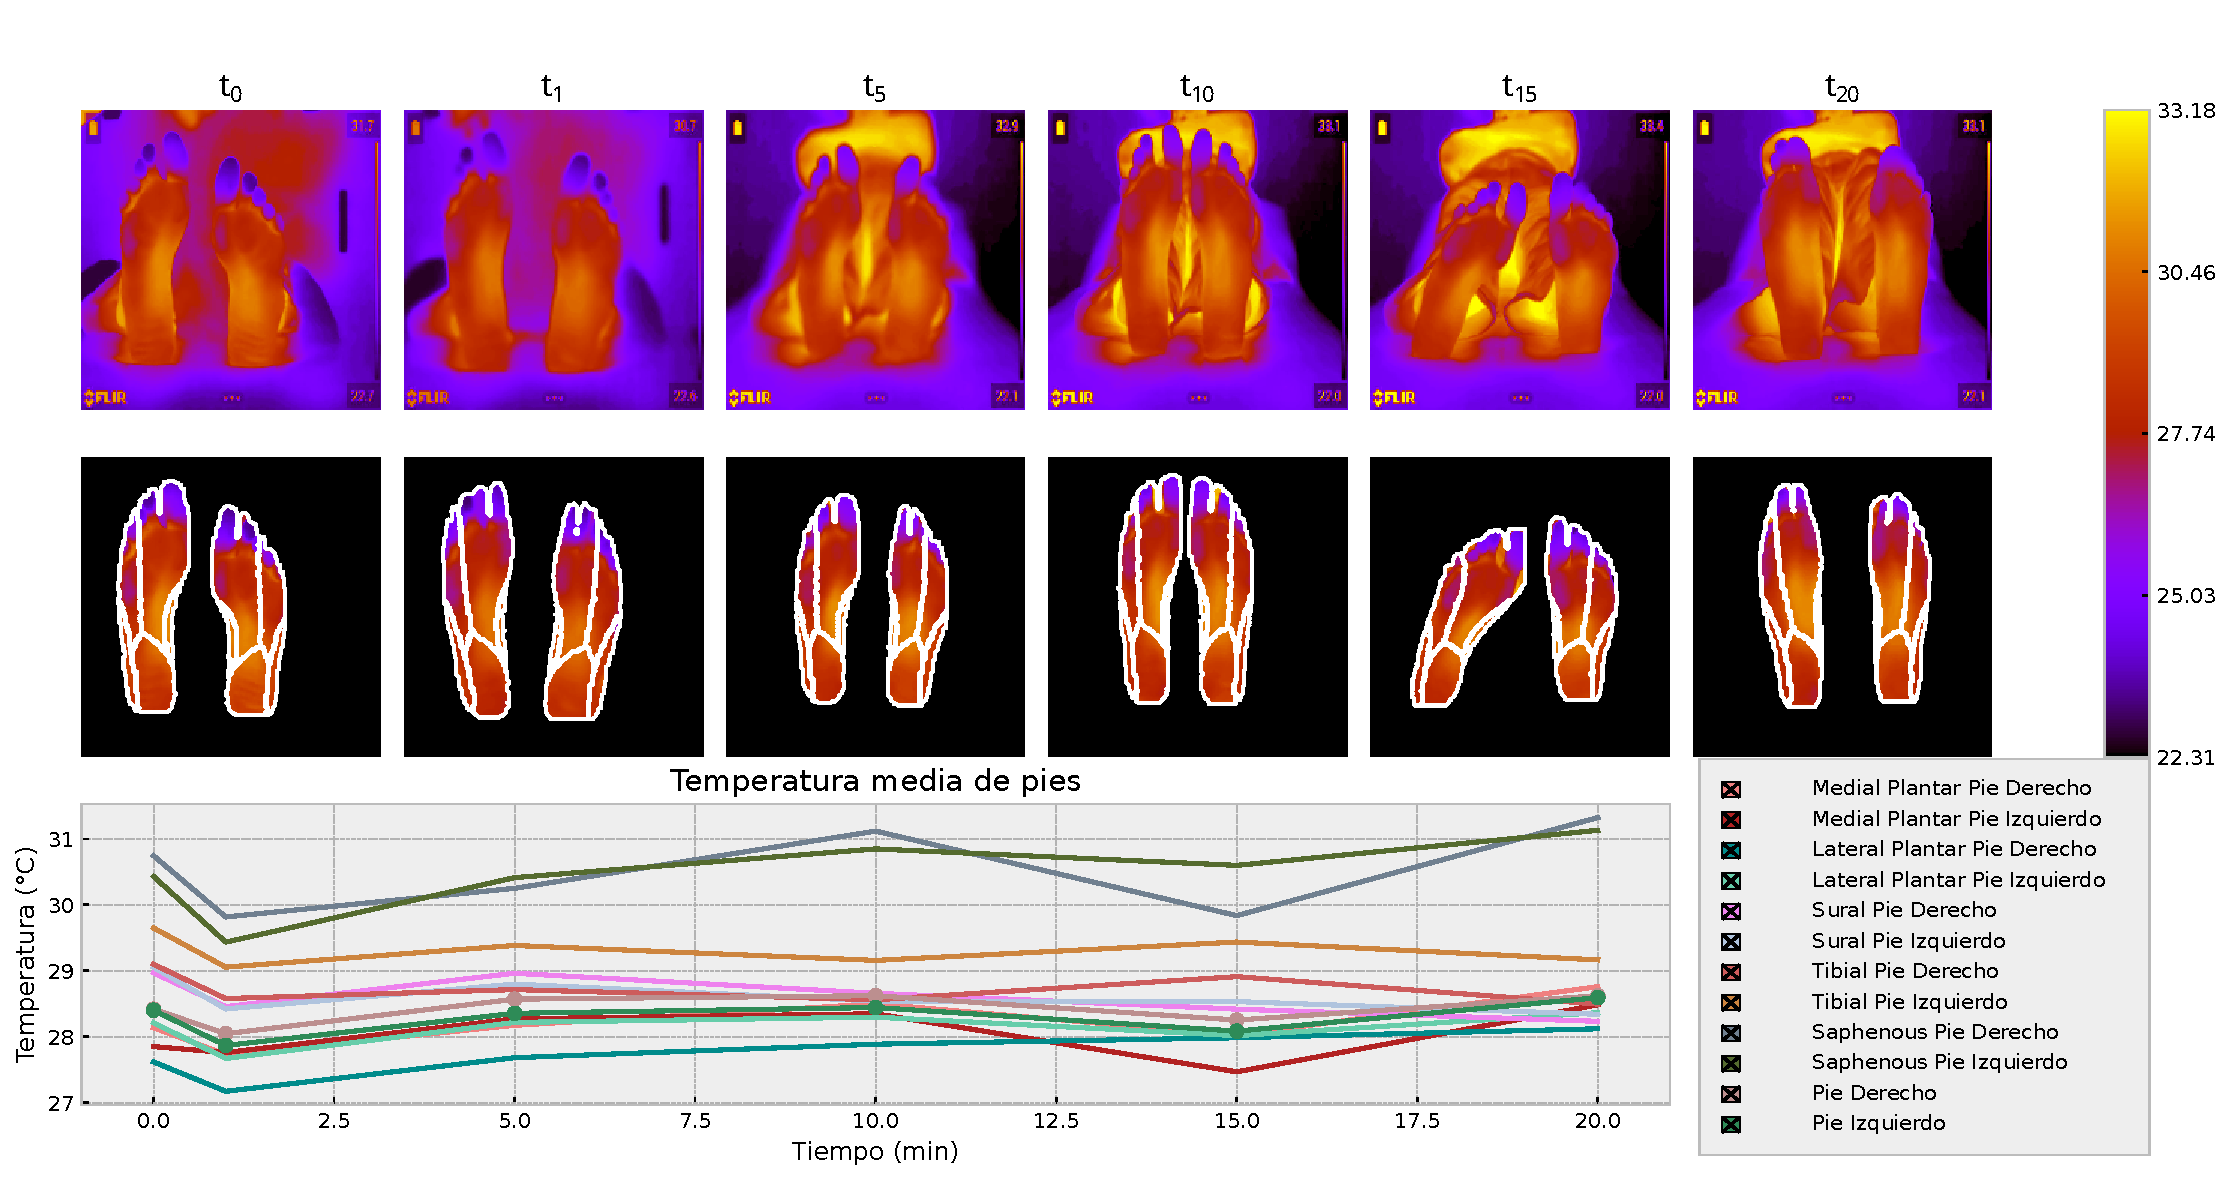
\includegraphics[width=0.87\linewidth]{Figures/report.pdf}
        % \caption{Data adquisition timeline}
        % \label{}
\end{figure}
    
\end{frame}



\section{Conclusions}

\begin{frame}{Conclusions}

\begin{itemize}
    \setlength\itemsep{1em}

        \item We propose an extension of the \textbf{Random Fourier Features} tailored for \textbf{spatial data}, introducing \textbf{CRFFg}—a data-driven approach that leverages gradient descent. 
        
        \item Our innovative extension effectively \textbf{enhances feature representation} within the skip connection of encoder-decoder models, particularly for semantic segmentation tasks. 
    
    \item We tested 15 model variations of three well-known  deep learning architectures for automatic feet semantic segmentation on \textbf{thermal images} that exhibit small \textbf{sample size and high variability} of regions of interest.
    


    \item We have introduced \textbf{quantitative measures} for enhancing \textbf{interpretability} in \textbf{semantic segmentation} models used in the medical field. 
    
    \item Our \textbf{approach quantifies the relevance location} of specific regions, the sensibility across multiple regions of interest, and their homogeneity.
\end{itemize}


\end{frame}

\begin{frame}{Future Work}

\begin{itemize}
    \setlength\itemsep{1em}
    \item \textbf{Analyzing the spectral representation} of the CRFFg to gain insights into underlying patterns, leading to a deeper understanding and potential improvements \cite{ZHANG202041}.
    
    \item Incorporating \textbf{Bayesian approximation} techniques to quantify uncertainties, model relationships between variables more accurately, and potentially uncover new strategies related to our CRFFg layer \cite{MILLER2022100598}.
    
    \item Employing \textbf{regularization techniques} to mitigate overfitting using the proposed interpretability measures \cite{chang2020mixupcam, 9506582}.

    \item Exploring alternative mappings for Random Fourier Features \cite{sutherland2015error} and the training of the scale $\sigma$ parameter, addressing class imbalance with different loss functions \cite{YEUNG2022102026}, and considering transformers instead of convolutions for better context capture \cite{azad2023advances}.
\end{itemize}
\end{frame}



\begin{frame}[allowframebreaks]{Academic Discussion}

\begin{itemize}
\setlength\itemsep{1em}

\item \small{Aguirre-Arango, J.C.; Álvarez-Meza, A.M.; Castellanos-Dominguez, G. Feet Segmentation for Regional Analgesia Monitoring Using Convolutional RFF and Layer-Wise Weighted CAM Interpretability. Computation 2023, 11, 113. https://doi.org/10.3390/computation11060113} \textbf{Q2/A2}
\item \small{Mejia-Zuluaga, Rafael, Juan Carlos Aguirre-Arango, Diego Collazos-Huertas, Jessica Daza-Castillo, Néstor Valencia-Marulanda, Mauricio Calderón-Marulanda, Óscar Aguirre-Ospina, Andrés Alvarez-Meza, and Germán Castellanos-Dominguez. "Deep Learning Semantic Segmentation of Feet Using Infrared Thermal Images." In Advances in Artificial Intelligence–IBERAMIA 2022: 17th Ibero-American Conference on AI, Cartagena de Indias, Colombia, November 23–25, 2022, Proceedings, pp. 342-352. Cham: Springer International Publishing, 2023.} \textbf{International Conference}
\item \small{A.D. Tobar, J.C. Aguirre, D.A. Cardenas-Pena, A.M. Alvarez-Meza, and C.G. Castellanos-Dominguez, "Hippocampus Segmentation using Patch-based Representation and ROC Label Enhancement," Engineering Letters, vol. 31, no. 2, pp504-510, 2023} \textbf{B}

\end{itemize}


\begin{table}[]
\begin{tabular}{ll}
\hline
\multicolumn{1}{c}{\textbf{Title}}  & \multicolumn{1}{c}{\textbf{Github repository}}   \\
\hline
Image segmentation library & \textcolor{blue}{\small{\href{https://github.com/UN-GCPDS/python-gcpds.image\_segmentation}{https://github.com/UN-GCPDS/python-gcpds.image\_segmentation}}} \\
CRFFg  layer               & \textcolor{blue}{\small{\href{https://github.com/aguirrejuan/ConvRFF}{https://github.com/aguirrejuan/ConvRFF}}}                       \\
Monitoring tool            & \textcolor{blue}{\small{\href{https://github.com/UN-GCPDS/FEET-GUI}{https://github.com/UN-GCPDS/FEET-GUI}}} \\
\hline
\end{tabular}
\end{table}

\end{frame}


\begin{frame}{Acknowledgments}

\begin{itemize}
    \setlength\itemsep{1em}
    \item \textit{``Herramienta de apoyo a la predicción de los efectos de anestésicos locales vía neuroaxial epidural a partir de termografía por infrarrojo" (Code 111984468021)} funded by MINCIENCIAS
    \item \textit{``Sistema prototipo de visión por computador utilizando aprendizaje profundo como soporte al monitoreo de zonas urbanas desde unidades aéreas no tripuladas" (Hermes Code 55261)}, funded by Universidad Nacional de Colombia.
\end{itemize}



\begin{center}
	{\Huge{\textbf{\textcolor[rgb]{0.00,0.00,1.00}{Thank you!}}}}\\
	\vspace{0.1cm}
	 Juan Carlos Aguirre Arango\\ \scriptsize{jucaguirrear@unal.edu.co}
\end{center}    
    
\end{frame}


\section{References}

\begin{frame}[allowframebreaks]%,noframenumbering]
\frametitle{References}
{\tiny 
\bibliographystyle{apalike}
\bibliography{References, References1,bibliography}
}
\end{frame}

\begin{frame}{Segmentation: Context information + Localization}
  Segmentation: Context information + Localization 
\begin{columns}
    \column{0.5\textwidth}
        \begin{figure}
        \centering \includegraphics[width=0.6\linewidth]{Figures/zebra1.jpg}
        \end{figure}  
    
    
    \column{0.5\textwidth}
            \begin{figure}
            \centering \includegraphics[width=0.4\linewidth]{Figures/zebra.jpg}
            \end{figure}
    
\end{columns}

Transformers have an infinite receptive field (High context).

Convolution has a local receptive field. Multiple layers increase the receptive field.   
\end{frame}



\begin{frame}{Quantitative Semantic Segmentation Results - Oxford Pet IIIt}
\begin{figure}
        \centering \includegraphics[width=1\linewidth]{Figures/results_oxford.pdf}
\end{figure}
\end{frame}





\begin{frame}[allowframebreaks]{Interpretability Results - ThermalFeet}

\begin{figure}
    \centering
    \includegraphics[width=0.85\linewidth]{Figures/fcn_best.pdf}
    \caption{FCN CRFFg S-M3 without data Augmentation}
\end{figure}
\framebreak

\begin{figure}
    \centering
    \includegraphics[width=0.79\linewidth]{Figures/resunet_best.pdf}
    \caption{ResUNet CRFFg S-M3 without data Augmentation}
\end{figure}
\framebreak

\begin{figure}
    \centering
    \includegraphics[width=0.79\linewidth]{Figures/unet_best.pdf}
    \caption{U-Net CRFFg S-M3 with data Augmentation}
\end{figure}

\end{frame}






\begin{frame}[allowframebreaks]{Interpretability Results - Oxford IIIt Pet}

\begin{figure}
        \centering
        \includegraphics[width=1\linewidth]{Figures/oxford_metrics.pdf}

\end{figure}


\framebreak
\begin{figure}[htbp]
  \centering
  \includegraphics[width=0.8\linewidth]{Figures/oxford_fcn_best.pdf}
  \caption{FCN S-M1}
\end{figure}

\framebreak
\begin{figure}[htbp]
  \centering
  \includegraphics[width=0.7\linewidth]{Figures/oxford_res_best.pdf}
  \caption{ResUNet S-M3}
\end{figure}


\framebreak
\begin{figure}[htbp]
  \centering
  \includegraphics[width=0.75\linewidth]{Figures/oxford_unet_best.pdf}
  \caption{U-Net S-M1}
\end{figure}


\end{frame}



\end{document}

